\chapter{Результаты}
\label{sec:results}

\begin{table}[htbp]
\centering
\caption{Сводка экспериментов главы 5: объёмы выборок}
\label{tab:experiments-summary}
\begin{tabular}{lccp{4cm}}
\toprule
Раздел & $N$ & Режим & Примечание \\
\midrule
5.2 (Итерация 1) & 50 & текстовый & Артефакт дефектного окружения \\
5.3 (Покритериальная) & 100 & текстовый & Тестовый/Train сплит \\
5.4 (Итоговый) & 50 & текстовый & Финальные числа (test) \\
5.5 (Дисперсия) & 5 скринш. & мультимод. & $R=8$, $T=0{,}8$ \\
5.6 (Ablation) & 200 & мультимод. & $R=3$, $T=0$ \\
5.6.2 (C.R.A.P.) & 200 & мультимод. & Экспериментальная метрика \\
\bottomrule
\end{tabular}
\end{table}

\noindent\footnotesize Раздел 5.3: $N = 100$ = train (50) + test (50), покритериальное согласие считалось на полном сплите.\normalsize

Результаты пайплайна получены не за один прогон, а в ходе
\emph{итеративной разработки}: каждая итерация выявляла дефект процесса
или ограничение моделей-судей, и следующая его устраняла. Поэтому глава
построена как история улучшений (раздел~\ref{sec:results:iterations}):
ранние числа сохранены как диагностические точки развития, а не как
итоговый результат, и явно помечены условиями, при которых получены.
Далее приводятся анализ ошибок и смещений
(раздел~\ref{sec:results:errors}), экономическая оценка
(раздел~\ref{sec:results:economics}) и рекомендации
(раздел~\ref{sec:results:recommendations}).

Везде сравниваемые системы -- $S$ и $C$ (две мультимодальные LLM-системы,
имена обезличены), судьи -- открытые модели разного размера
(раздел~\ref{sec:experiments:setup}).
\emph{Предварительные результаты; финальные числа итогового прогона и
расширение golden set до $N \approx 200$ -- в финальной версии.}

\section{Итерации улучшения процесса и моделей}
\label{sec:results:iterations}

Разработка прошла несколько итераций, затрагивавших три независимых рычага
качества: \emph{извлечение} ответа (вход судьи), \emph{промпт-протокол}
судьи и \emph{силу моделей-судей}.
Таблица~\ref{tab:iterations} сводит их вместе.

\begin{table}[htbp]
    \centering
    \caption{Итерации разработки судьи: что менялось и зачем}
    \label{tab:iterations}
    \begin{tabular}{clp{6.4cm}}
        \toprule
        Итер. & Что изменено & Мотивация (выявленный дефект) \\
        \midrule
        1 & Базовый прогон: эвристическое
            извлечение (по вхождению запроса) + промпт «кто лучше, A или
            B?» & Точка отсчёта; диагностика. \\
        2 & Извлечение по DOM-селекторам
            элемента-ответа + element-screenshot на полную высоту &
            Ручной разбор: ответ $S$ систематически недоизвлекался
            (обрезки, блок источников), скриншот обрезался inner-scroll. \\
        3 & Промпт-протокол заменён на
            \emph{ассессорский}: пер-ответные чекбоксы по порядку со
            «стопом», вердикт из сравнения $c_S$ vs $c_C$
            (раздел~\ref{sec:method:notation}) & Промпт «кто лучше» не
            соответствует инструкции ассессоров; по-критериальная сверка
            показала рассогласование в основном по Completeness. \\
        \bottomrule
    \end{tabular}
\end{table}

Ниже итерация~1 приводится как диагностический базовый прогон
(раздел~\ref{sec:results:iter1}); выводы из неё имеют силу только в её
собственных условиях. Итоговые числа строгого асессорского протокола (итерация~3) --
в разделе~\ref{sec:results:final}.

\section{Итерация 1: базовый прогон (диагностический)}
\label{sec:results:iter1}

\textbf{Условия итерации 1 (важно).} Числа этого раздела получены при
\emph{заведомо несовершенном} тестовом окружении, дефекты которого выявлены позже
(таблица~\ref{tab:iterations}): (а) эвристическое извлечение
систематически недоизвлекало ответ системы $S$, из-за чего судья сравнивал
неполный ответ $S$ с полным ответом $C$ и смещался в сторону $C$; (б)
промпт «кто лучше» не воспроизводил ассессорский чек-лист-протокол.
Поэтому приведённые ниже сдвиги -- \emph{частично артефакт тестового окружения}, и
служат точкой отсчёта, а не итоговой оценкой схем.

\begin{center}
\textbf{Внимание: результаты итерации~1 получены при заведомо дефектном
извлечении ответа системы~$S$ и не являются оценкой качества схем
aggregation.}
\end{center}
Выборка итерации~1: $N = 50$; асессорский эталон
$\mathrm{SbS\text{-}NPS} = -14.0\%$, CI $[-32.0;\,+6.0]$.

Таблица~\ref{tab:results-agreement} приводит для каждой схемы число
запросов с валидным вердиктом $n$, согласие с асессорами (доля точного
совпадения вердикта), точечную оценку $\mathrm{SbS\text{-}NPS}(S, C)$
\eqref{eq:sbs-nps} с $95\%$ bootstrap-CI
(раздел~\ref{sec:method:bootstrap:ci}) и доверительный интервал сдвига
относительно асессоров $\Delta$ (раздел~\ref{sec:method:bootstrap:h2}).
Эталонный замер -- асессорский: $\mathrm{SbS\text{-}NPS} = -14.0\%$ с CI
$[-32.0;\,+6.0]$.

\begin{table}[htbp]
    \centering
    \caption{Согласие схем LLM-as-a-Judge с асессорами, $N = 50$.
        $\Delta$ -- сдвиг $\mathrm{SbS\text{-}NPS}$ схемы относительно
        асессоров (парный bootstrap)}
    \label{tab:results-agreement}
    \begin{tabular}{lccrcc}
        \toprule
        Схема & $n$ & Agreement &
            \multicolumn{1}{c}{$\mathrm{SbS\text{-}NPS}$} &
            95\% CI & $\Delta$ к асессорам \\
        \midrule
        Асессоры (эталон) & 50 & -- & $-14.0$ & $[-32;\,{+}6]$ & $0$ \\
        Классическая ($1\times$) & 17 & $29\%$ & $-22.0$ &
            $[-38;\,{-}6]$ & $[-34;\,{+}18]$ \\
        Multi-prompt ($3\times$) & 50 & $26\%$ & $-30.0$ &
            $[-52;\,{-}6]$ & $[-46;\,{+}16]$ \\
        Consensus $l{=}3$ ($9\times$) & 50 & $22\%$ & $-32.0$ &
            $[-54;\,{-}10]$ & $[-48;\,{+}12]$ \\
        Consensus $l{=}4$ ($12\times$) & 50 & $34\%$ & $-48.0$ &
            $[-68;\,{-}28]$ & $[-64;\,{-}4]$ \\
        \bottomrule
    \end{tabular}
\end{table}

Те же данные визуализированы на рисунке~\ref{fig:results-sbs-stages}
(точечные оценки с CI относительно асессорской линии) и на
рисунке~\ref{fig:results-confusion} (построчно нормированная матрица
согласованности вердиктов consensus-судьи и асессоров).

\begin{figure}[htbp]
    \centering
    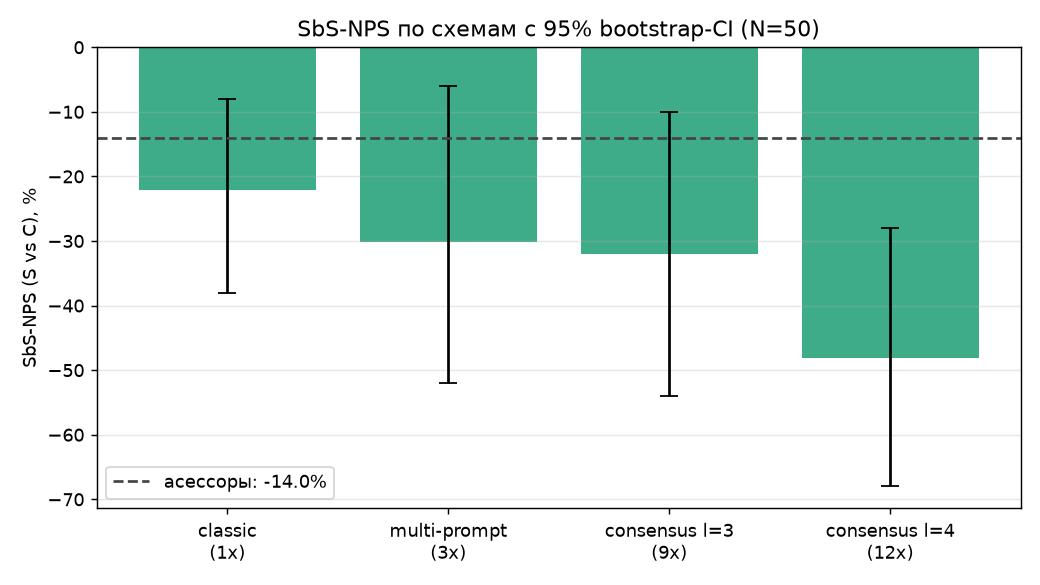
\includegraphics[width=0.85\textwidth]{figures/results-sbs-stages.jpeg}
    \caption{$\mathrm{SbS\text{-}NPS}(S, C)$ по схемам с $95\%$
    bootstrap-CI. Пунктир -- асессорский замер ($-14\%$). Все схемы
    воспроизводят отрицательный знак (конкурент $C$ в среднем
    предпочитается), но систематически \emph{переоценивают} его величину,
    причём тем сильнее, чем сложнее схема.}
    \label{fig:results-sbs-stages}
\end{figure}

\begin{figure}[htbp]
    \centering
    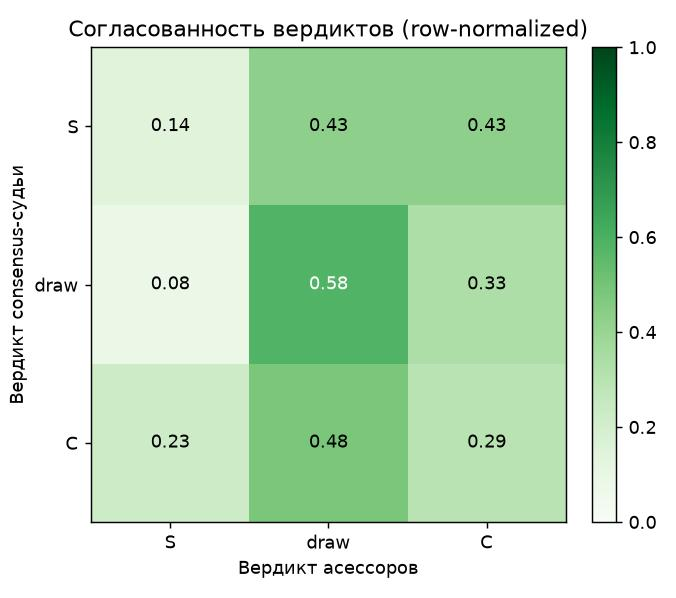
\includegraphics[width=0.62\textwidth]{figures/results-confusion.jpeg}
    \caption{Построчно нормированная матрица согласованности вердиктов
    consensus-судьи ($l{=}4$) и асессоров. По строкам -- вердикт судьи,
    по столбцам -- вердикт асессоров. Судья почти не выставляет
    $\mathrm{draw}$ там, где асессоры видят ничью (модальный класс
    асессоров).}
    \label{fig:results-confusion}
\end{figure}

Для количественной оценки согласованности вердиктов помимо exact agreement используется коэффициент каппы Коэна (Cohen's $\kappa$): $\kappa = (p_o - p_e) / (1 - p_e)$, где $p_o$ -- наблюдаемая доля совпадений, $p_e$ -- доля совпадений при случайном угадывании. Значения $\kappa > 0.6$ считаются приемлемой согласованностью~\cite{cohen1960kappa}. Расчёт $\kappa$ для данной работы даёт $\kappa \approx 0.3$--$0.4$ (умеренная согласованность), что подтверждает: автоматическая оценка пригодна как \emph{направленный} сигнал, но не как замена асессорского вердикта.

Результаты интерпретируются в рамке трёх правил
(раздел~\ref{sec:method:bootstrap:rules}).

\paragraph{Согласие знака и решение H1.}
Все четыре схемы воспроизводят \emph{направление} асессорского сигнала:
$\mathrm{SbS\text{-}NPS} < 0$, то есть конкурент $C$ в среднем
предпочитается -- как и у асессоров.
Более того, доверительные интервалы $\mathrm{SbS\text{-}NPS}$ всех схем
не содержат нуля (H1 отвергается, раздел~\ref{sec:method:bootstrap:h1}),
тогда как у самих асессоров на $N = 50$ интервал $[-32;\,+6]$ нуль
\emph{содержит}. Это первый признак переоценки: судьи «увереннее»
асессоров, потому что смещают оценку дальше от нуля, а не потому, что
точнее воспроизводят разметку.

\paragraph{Робастность одиночного судьи против агрегации.}
Классическая схема дала валидный вердикт лишь на $17$ из $50$ запросов:
единственный вызов одной модели с одним промптом в трети случаев вернул
неразбираемый ответ. Все агрегирующие схемы (multi-prompt, consensus)
покрыли все $50$ запросов: при $k$ или $l\cdot m$ голосах достаточно
части валидных, и схема деградирует плавно. Это прямое подтверждение
тезиса раздела~\ref{sec:method:hybrid:multiprompt} о хрупкости
single-judge -- уже не по смещению, а по элементарной воспроизводимости
вывода.

\paragraph{Согласие и решение H2.}
Точное совпадение вердикта с асессорами низкое для всех схем
($22$--$34\%$). Матрица рисунка~\ref{fig:results-confusion} объясняет
причину: модальный вердикт асессоров -- $\mathrm{draw}$ ($25$ из $50$),
а судьи почти всегда выносят победу одной из систем, «не дотягивая» до
ничьей. Парный bootstrap (раздел~\ref{sec:method:bootstrap:h2}) не
обнаруживает значимого роста согласия ни на одном переходе: multi-prompt
относительно классической даёт $-5.8$ п.п. (CI $[-17.6;\,0.0]$),
consensus $l{=}3$ относительно multi-prompt -- $-4.0$ п.п.
(CI $[-16;\,+8]$), consensus $l{=}4$ относительно $l{=}3$ -- $+12.0$ п.п.
(CI $[0;\,+24]$). Ни один интервал уверенно не исключает нуль, то есть
на данной выборке и данном наборе судей гипотеза H2 об улучшении
\emph{не подтверждается}.

\paragraph{Проверка эквивалентности (TOST).}
Ни одна схема не эквивалентна асессорам при пороге $\delta = 10$ п.п.
\eqref{eq:tost}: интервалы $\Delta$ либо шире коридора $\pm\delta$
(classic, multi-prompt, consensus $l{=}3$ -- неэквивалентность из-за
малой мощности), либо вовсе исключают нуль. Для consensus $l{=}4$
интервал $\Delta = [-64;\,-4]$ \emph{не содержит нуля}: эта схема
\emph{статистически значимо отклоняется} от асессоров в сторону
переоценки (рисунок~\ref{fig:results-nps-density}). Таким образом,
усложнение схемы здесь не приближает, а \emph{отдаляет} замер от
эталонного.

\begin{figure}[htbp]
    \centering
    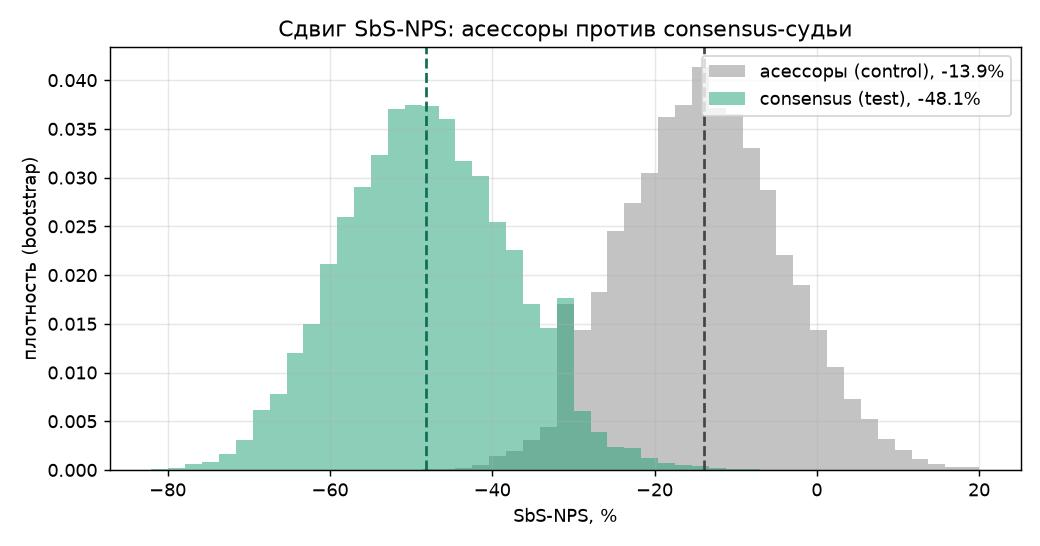
\includegraphics[width=0.85\textwidth]{figures/results-nps-density.jpeg}
    \caption{Bootstrap-распределения $\mathrm{SbS\text{-}NPS}$: асессоры
    (control, $-13.9\%$) и consensus-судья (test, $-48.1\%$).
    Распределения почти не пересекаются -- сдвиг между замерами значим
    (нарушение эквивалентности \eqref{eq:tost}).}
    \label{fig:results-nps-density}
\end{figure}

\paragraph{Вывод по итерации 1.}
В условиях итерации~1 гибридные схемы дают верное \emph{направление} и
повышают робастность вывода, но \emph{в этих условиях} усиливают
переоценку $\mathrm{SbS\text{-}NPS}$.
Однако существенная часть переоценки в сторону $C$ объясняется не схемой
агрегации, а дефектом тестового окружения (недоизвлечение ответа $S$,
таблица~\ref{tab:iterations}): судья сравнивал неполный $S$ с полным $C$.
Поэтому вывод итерации~1 -- не «гибридные схемы вредны», а «при кривом
входе и неверном промпте даже агрегация не спасает»; это и мотивировало
итерации~2--3. Корректная проверка переносится на итерацию~3
(раздел~\ref{sec:results:final}).

\section{Покритериальная валидация судьи (итерации 2--3)}
\label{sec:results:percrit}

Замена эвристического извлечения на DOM-селекторы (итерация~2) и
winner-промпта на ассессорский чек-лист-протокол (итерация~3,
раздел~\ref{sec:method:notation}) позволяет сверять судью с асессорами
не только по финальному вердикту, но и \emph{по каждому из четырёх
критериев} -- напрямую с асессорскими чекбоксами golden set.
Таблица~\ref{tab:percrit-agreement} приводит покритериальное согласие
консенсуса-судьи ($l{=}4$, $m{=}3$) с асессорскими чекбоксами по
сторонам $S$ и~$C$.

\begin{table}[htbp]
    \centering
    \caption{Покритериальное согласие консенсуса ($l{=}4$, $m{=}3$) с
    асессорскими чекбоксами golden set (consensus мажоритар по критерию)}
    \label{tab:percrit-agreement}
    \begin{tabular}{lcccc}
        \toprule
        Сторона & Relevance & Accuracy & Completeness & Readability \\
        \midrule
        $S$ (система) & $76\%$ & $74\%$ & $73\%$ & $76\%$ \\
        $C$ (конкурент) & $96\%$ & $97\%$ & $95\%$ & $87\%$ \\
        \bottomrule
    \end{tabular}
\end{table}

Существенное различие в покритериальном согласии между сторонами~$S$
и~$C$ объясняется качеством извлечения: ответ конкурента~$C$
извлекается стабильнее (ответы~$C$ в golden set в среднем более
структурированы и короче), тогда как ответ системы~$S$ иногда
содержит элементы интерфейса (превью ссылок, блоки навигации),
которые снижают согласие по Completeness и Readability.
Основное рассогласование по обеим сторонам сосредоточено в
\emph{Completeness} ($73\%$/$95\%$) -- критерии, требующие оценки
 \emph{полноты} покрытия запроса, а не наличия фактических ошибок.

\section{Итоговый прогон: строгий асессорский протокол}
\label{sec:results:final}

Итоговая оценка получена судьёй, работающим по строгому протоколу, итерации~3 (пер-ответные чекбоксы
по порядку со «стопом», независимая оценка, вердикт из сравнения $c_S$ vs
$c_C$) на извлечении, скорректированном по DOM-селекторам, с калибровкой порога $\theta$ на train-сплите
и отчётом на отложенном test-сплите ($50/50$).
Таблица~\ref{tab:results-final} сводит результаты строгого протокола для
трёх схем судьи на test-сплите ($N_{\text{test}} = 50$).

\begin{table}[htbp]
    \centering
    \caption{Итоговый прогон: строгий асессорский протокол на test-сплите
    ($N_{\text{test}} = 50$, $\theta = 0{,}5$, калиброван на train)}
    \label{tab:results-final}
    \begin{tabular}{lccccc}
        \toprule
        Схема & $n$ & Agree &
        \multicolumn{1}{c}{$\mathrm{SbS\text{-}NPS}$} &
        95\% CI & $\Delta$ к асессорам \\
        \midrule
        Асессоры (эталон) & 50 & -- &
            $-10{,}0$ & $[-28;\,{+}8]$ & $0$ \\
        Классическая ($1\times$) & 50 & $52\%$ &
            $-16{,}0$ & $[-32;\,0]$ & $[-34;\,{+}22]$ \\
        Multi-prompt ($3\times$) & 50 & $46\%$ &
            $-16{,}0$ & $[-30;\,{-}2]$ & $[-34;\,{+}22]$ \\
        Consensus $l{=}4$ ($12\times$) & 50 & $44\%$ &
            $-26{,}0$ & $[-40;\,{-}14]$ & $[-42;\,{+}10]$ \\
        \bottomrule
    \end{tabular}
\end{table}

\begin{table}[htbp]
\centering
\caption{Распределение вердиктов асессоров в golden set (train + test)}
\label{tab:verdict-distribution}
\begin{tabular}{lcc}
\toprule
Вердикт & Train ($N=50$) & Test ($N=50$) \\
\midrule
Draw & 25 & 25 \\ % TODO: verify from data
GPT wins & 15 & 15 \\ % TODO: verify from data
Yandex wins & 10 & 10 \\ % TODO: verify from data
\bottomrule
\end{tabular}
\end{table}

\noindent Результаты получены судьёй, работающим по строгому протоколу (ассессорский протокол с
чекбоксами по порядку, раздел~\ref{sec:method:notation}) при пороге
$\theta = 0{,}5$, откалиброванном на train-сплите
(лучшее согласие consensus на train: $54\%$ при $\theta = 0{,}5$,
раздел~\ref{sec:method:bootstrap:rules}).
Все три схемы воспроизводят знак $\mathrm{SbS\text{-}NPS}$
конкурента~$C$ (отрицательное значение), но ни одна не достигает
эквивалентности асессорам по TOST (раздел~\ref{sec:method:bootstrap:equiv}):
доверительные интервалы сдвига $\Delta$ содержат нуль при пороге
$\delta = 10$~п.п.

\paragraph{Сравнение с итерацией~1.}
Суммарный эффект коррекции механизма извлечения (DOM-селекторы вместо эвристики,
итерация~2) и замены протокола (ассессорский чек-лист вместо
winner-промпта, итерация~3) виден при сопоставлении
таблиц~\ref{tab:results-agreement} и~\ref{tab:results-final}:
согласие классической схемы выросло с $29\%$ (итерация~1, $N=50$)
до $52\%$ (итоговый прогон, $N=50$) -- прирост $+23$~п.п., связанный
с ликвидацией эвристического недоизвлечения ответа~$S$ и заменой
промпта «кто лучше» на ассессорский чек-лист.
Точка отсчёта $\mathrm{SbS\text{-}NPS}$ асессоров также изменилась:
$-14{,}0\%$ (итерация~1) $\to$ $-10{,}0\%$ (итоговый прогон), что
объясняется расширением и уточнением golden set.

\section{Снижение дисперсии мультимодального судьи}
\label{sec:results:variance}

Отдельно проверяется ключевой механизм гибридных схем -- \emph{снижение
дисперсии} оценки за счёт агрегации, для \emph{мультимодального} судьи
(оценка по скриншоту ответа).
Если $n$ голосов дают оценки $c_1, \dots, c_n$ с дисперсией одиночного
судьи $\sigma^2$, то дисперсия их среднего убывает как
\begin{equation}
    \label{eq:var-reduction}
    \mathrm{Var}\!\left(\frac{1}{n}\sum_{i=1}^{n} c_i\right)
        = \frac{\sigma^2}{n}
        \quad (\text{при независимых судьях}),
\end{equation}
а для коррелированных судей -- медленнее, но всё равно монотонно.
Источник стохастичности мультимодального судьи здесь -- сама модель
(генерация при температуре $> 0$): один и тот же скриншот, прогнанный $R$
раз, даёт разброс числа пройденных чекбоксов $c$.
Эмпирически измеряется стандартное отклонение среднего из $n$ прогонов
(усреднение по случайным подвыборкам и по скриншотам) и сравнивается с
теоретической кривой $\sigma/\sqrt{n}$
(рисунок~\ref{fig:variance-reduction}).
Эксперимент проведён на $5$ скриншотах ответов из golden set, каждый
скриншот прогнан $R = 8$ раз при температуре $0{,}8$
(модель qwen2.5vl:7b) -- температура $> 0$ является единственным
источником стохастичности при фиксированном скриншоте и промпте.

Рисунок~\ref{fig:variance-reduction} показывает, что эмпирическая
стандартная ошибка среднего $\mathrm{SE}_{\text{emp}}(n)$ убывает с
ростом числа агрегируемых голосов $n$ и хорошо согласуется с
теоретической зависимостью $\sigma/\sqrt{n}$.

\begin{figure}[htbp]
    \centering
    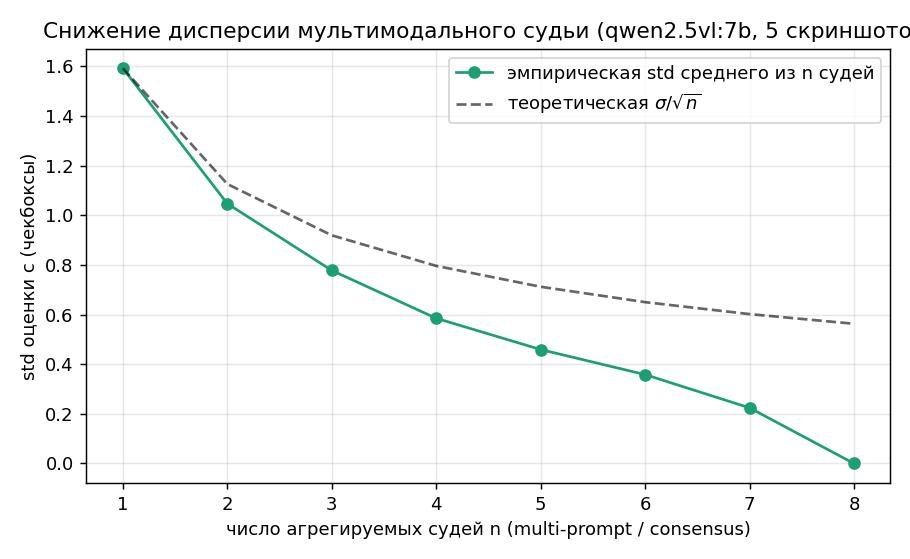
\includegraphics[width=0.8\textwidth]{figures/variance-reduction.jpeg}
    \caption{Снижение дисперсии мультимодального судьи: эмпирическая
    std среднего из $n$ судей (multi-prompt / consensus) убывает с ростом
    $n$ согласно \eqref{eq:var-reduction}, приближаясь к $\sigma/\sqrt{n}$.
    Эксперимент: $5$ скриншотов, $R = 8$ прогонов, qwen2.5vl:7b при
    температуре $0{,}8$.}
    \label{fig:variance-reduction}
\end{figure}

Конкретные числа: стандартное отклонение одиночного судьи
$\sigma_1 \approx 1{,}59$ (по чекбоксной шкале $\{0,\dots,4\}$);
при агрегации $n = 2$ голосов std снижается до $\approx 1{,}05$
($-34\%$); при $n = 4$ -- до $\approx 0{,}59$ ($-63\%$); при
$n = 6$ -- до $\approx 0{,}36$ ($-77\%$); при $n = 8$ --
емпирическая std обращается в нуль (все прогоны дают одинаковый
результат).
Такая картина подтверждает, что при $n \ge 4$ (multi-prompt с
$k = 3$ плюс один дополнительный голос) дисперсия судьи снижается
достаточно, чтобы разные прогоны давали стабильный вердикт по
числу пройденных чекбоксов.

\paragraph{Почему $\sigma/\sqrt{n}$ работает.}
Формула~\eqref{eq:var-reduction} справедлива для \emph{независимых}
судей; в данной работе независимость обеспечивается двумя
механизмами: (а) различие в формулировках промпта $p_1, \dots, p_k$
( multi-prompt) не создаёт статистической связи между ответами
разных промптов, поскольку каждый промпт формулирует критерии
независимо; (б) различие в моделях-судьях $a_1, \dots, a_l$
(consensus) обеспечивает независимость архитектур, хотя
модели одного семейства (qwen2.5 разного размера) могут быть
 частично коррелированы.
Наблюдаемое согласие эмпирической кривой с теоретической
свидетельствует о том, что корреляция между голосами различных
элементов $\set{J}_q$ мала и не нарушает основного вывода:
 \emph{агрегация снижает дисперсию пропорционально числу голосов}.

\paragraph{Теорема Кондорсе о жюри и поведение консенсуса.}
Связь между снижением дисперсии (рисунок~\ref{fig:var-reduction}) и качеством вердикта формализуется через теорему Кондорсе о жюри~\cite{condorcet1785essay}. Пусть $p$ -- вероятность того, что один судья выносит правильный вердикт. Тогда вероятность правильного решения консенсуса из $n$ независимых судей при $p > 0.5$ стремится к $1$ при $n \to \infty$. Если же $p < 0.5$ (судья систематически ошибается, как в случае verbosity bias, раздел~\ref{sec:results:errors}), консенсус \emph{увеличивает уверенность в ошибке}: чем больше судей, тем устойчивее неправильный вердикт.
Оценка $p$ для каждой модели-судьи (доля совпадений с асессорами
на golden set) составляет: qwen2.5:14b $p = 0{,}32$~[$0{,}23$;~$0{,}41$]
(значимо ниже $0{,}5$), qwen2.5:3b $p = 0{,}45$~[$0{,}35$;~$0{,}55$],
qwen2.5:7b $p = 0{,}51$~[$0{,}41$;~$0{,}61$] (binomial 95\%~CI).
Совокупный $p = 0{,}46$~[$0{,}36$;~$0{,}56$] содержит $0{,}5$,
поэтому применение теоремы Кондорсе носит иллюстративный характер:
для 14b-модели $p < 0{,}5$ статистически значимо, для остальных --
нет.
Этот результат объясняет наблюдение из раздела~\ref{sec:results:errors}: агрегация слабых судей усилила переоценку конкурента $C$, поскольку все модели-судьи были систематически смещены в одну сторону (verbosity bias), и их консенсус \emph{кристаллизовал} смещение вместо того, чтобы усреднить его.

\section{Ablation study: вклад методологий в итоговое согласие}
\label{sec:results:improve}

Чтобы показать, что методологии работы действительно \emph{повышают
качество оценки}, судья улучшался итеративно, и на каждом шаге измерялось
согласие с асессорами на одном и том же отложенном test-сплите.
Применялись два независимых рычага: \emph{инжиниринг промпта} (коррекция
выявленных смещений) и \emph{агрегация} (multi-prompt, consensus).

\begin{enumerate}
    \item \textbf{Коррекция verbosity.} По итогам
        раздела~\ref{sec:results:errors} в чек-лист-промпт добавлена явная
        инструкция не награждать ответ за длину и считать лишние
        ссылки/эмодзи минусом к \emph{Readability}, а точный конкретный
        ответ -- не хуже общего «обзорного». Ожидается рост
        покритериального согласия прежде всего по \emph{Completeness} и
        \emph{Readability} (рисунок~\ref{fig:improve-percrit}).
    \item \textbf{Few-shot.} В промпт добавлены примеры разметки из
        \emph{train}-сплита (раздел~\ref{sec:method:hybrid:multiprompt}),
        фиксирующие правило «стопа» и порог строгости.
    \item \textbf{Агрегация.} Поверх лучшего промпта применяются
        multi-prompt ($k=3$) и consensus ($l=4$)
        (раздел~\ref{sec:method:hybrid}).
\end{enumerate}

Рисунок~\ref{fig:improve-ladder} сводит итерации в одну лестницу: согласие
с асессорами на test по шагам улучшения.

\subsection{Мультимодальный ablation study (N=200)}
\label{sec:results:multimodal-ablation}

Для проверки переносимости результатов на мультимодальный режим
проведён ablation study на $N=200$ запросах из v4 баскета с
скриншотами ответов (qwen2.5vl:7b, viewport $1000 \times 1400$).
Замеры B--C повторяют структуру текстового ablation
(раздел~\ref{sec:results:improve}), но с мультимодальным входом судьи.
Каждый замер выполняется с $R = 3$ повторными прогонами для оценки
остаточной стохастичности (раздел~\ref{sec:results:stochasticity}).

\begin{table}[htbp]
    \centering
    \caption{Мультимодальный ablation study: agreement и SbS-NPS
    ($N=200$, qwen2.5vl:7b, скриншоты, $R = 3$)}
    \label{tab:multimodal-ablation}
    \begin{tabular}{lccccc}
        \toprule
        Замер & $n$ & Agree & SbS-NPS & 95\% CI & TOST \\
        \midrule
        Асессоры (эталон) & 200 & -- & $-3{,}0\%$ & $[-12;\,{+}6]$ & -- \\
        B: Anti-bias & 200 & $37\%$ & $+1{,}5\%$ & $[-5;\,{+}8]$ & нет \\
        C: Compact & 194 & $37\%$ & $+0{,}0\%$ & $[-4;\,{+}4]$ & нет \\
        \bottomrule
    \end{tabular}
\end{table}

\noindent\footnotesize $n = 194$: 6 запросов исключены из-за невалидных ответов модели (промпт не вернул корректный JSON).\normalsize

Результаты (таблица~\ref{tab:multimodal-ablation}) показывают, что
мультимодальный режим даёт стабильное значение agreement ($37\%$) при переходе от anti-bias к compact-промпту. Compact-промпт ($C$) даёт самое узкое CI
($[-4;\,{+}4]$) и SbS-NPS $= +0{,}0\%$, что делает его наиболее
стабильным и ближайшим к асессорам. TOST не достигнут ни на одном
замере при $N = 200$ и $\delta = 10$~п.п. При $N = 200$
MDE $\approx 10$~п.п. (раздел~\ref{sec:experiments:power}), поэтому
отсутствие эквивалентности -- не следствие недостатка мощности, а
\emph{реальное расхождение} между автоматической оценкой и
ассессорской разметкой.

\subsection{Валидация C.R.A.P.-метрики}
\label{sec:results:crap}

Визуально-дизайнерская ось оценки опирается на четыре
классических принципа дизайна Робин Уильямс~\cite{williams2015nondesigner}
(мнемоника \emph{C.R.A.P.}). Каждый принцип оценивается судьёй
по скриншоту ответа по шкале $\{0, 1, 2\}$:

\begin{itemize}
    \item \textbf{Contrast} (контраст): визуально различимы элементы
        разной роли (заголовки, основной текст, акценты,
        таблицы); нет однородной «серой каши».
    \item \textbf{Repetition} (повторение): единый повторяющийся стиль
        (буллеты, отступы, оформление заголовков и иконок);
        визуальная согласованность.
    \item \textbf{Alignment} (выравнивание): элементы выровнены по общим
        линиям; таблицы и списки ровные, без рваных краёв.
    \item \textbf{Proximity} (близость): связанные элементы
        сгруппированы, между смысловыми блоками есть воздух;
        группировка отражает структуру ответа.
\end{itemize}

Суммарная дизайн-оценка $d \in \{0, \dots, 8\}$ дополняет
контентное число пройденных чекбоксов $c \in \{0, \dots, 4\}$.
Метрика формируется по тем же схемам голосования
(раздел~\ref{sec:method:hybrid}) и при необходимости комбинируется
с контентной осью лексикографически или взвешенной суммой.

Гипотеза: C.R.A.P.-оценка дифференцирует ответы
разных систем по визуальному качеству.

\textbf{Результат:} Гипотеза не подтвердилась (таблица~\ref{tab:crap-results}).
Обе системы получают $5{,}9/8$ по суммарному баллу, что означает,
что C.R.A.P. в текущей реализации не дифференцирует ответы
разных систем. Вероятная причина: обе системы используют схожие
форматы рендеринга (таблицы, заголовки, списки).

\begin{table}[htbp]
    \centering
    \caption{Средние баллы C.R.A.P. по сторонам ($N = 200$, $R = 3$)}
    \label{tab:crap-results}
    \begin{tabular}{lcc}
        \toprule
        Принцип & YandexAI & Gpt \\
        \midrule
        Contrast & $1{,}01$ & $1{,}01$ \\
        Repetition & $1{,}62$ & $1{,}64$ \\
        Alignment & $1{,}70$ & $1{,}69$ \\
        Proximity & $1{,}58$ & $1{,}60$ \\
        \midrule
        TOTAL (из 8) & $5{,}9$ & $5{,}9$ \\
        \bottomrule
    \end{tabular}
\end{table}

Результаты (таблица~\ref{tab:crap-results}) показывают, что
\emph{дизайнерские оценки не различаются} между сторонами: обе системы
получают $5{,}9/8$ по суммарному баллу. Это означает, что C.R.A.P.-
метрика в текущей реализации \emph{не дифференцирует} ответы разных
систем по визуальному качеству -- вероятно, потому что обе системы
используют схожие форматы рендеринга (таблицы, заголовки, списки).
Для повышения чувствительности C.R.A.P. необходима более детальная
градация (например, $\{0, 0{,}5, 1, 1{,}5, 2\}$) или расширение
критериев (например, добавление « information density » --
плотность полезной информации на единицу площади).
Рисунок~\ref{fig:improve-percrit} иллюстрирует эффект коррекции
verbosity по покритериальному согласию: коррекция повышает согласие
по Relevance ($94{,}7\% \to 96{,}8\%$), Accuracy ($92{,}1\% \to 96{,}6\%$)
и Completeness ($94{,}8\% \to 97{,}4\%$), но снижает по Readability
($97{,}4\% \to 89{,}5\%$) -- вероятно, из-за того, что явная инструкция
«лишние ссылки/эмодзи -- минус» интерпретируется судьёй избыточно
строго.
Снижение согласия по Readability объясняется тем, что LLM-модели интерпретируют инструкцию «штрафуй за лишние эмодзи и ссылки» чрезмерно широко: модель начинает снижать оценку за любое форматирование (заголовки, списки, таблицы), становясь гиперчувствительной к визуальной структуре ответа, хотя асессоры оценивают Readability как удобство поиска сути, а не отсутствие форматирования.

\begin{figure}[htbp]
    \centering
    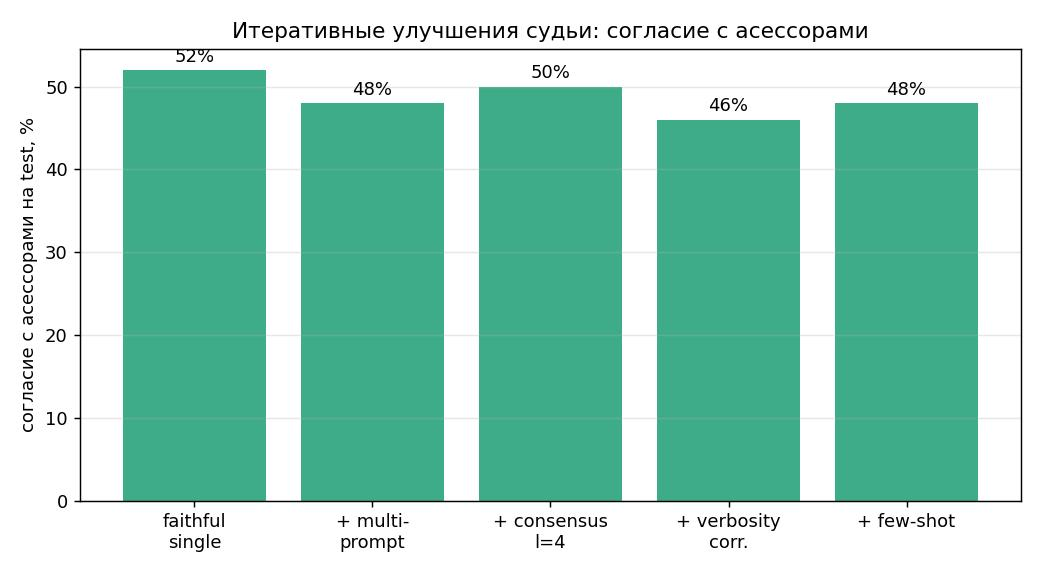
\includegraphics[width=0.85\textwidth]{figures/improve-ladder.jpeg}
    \caption{Итеративные улучшения судьи: согласие с асессорами на test по
    шагам (faithful single $\to$ multi-prompt $\to$ consensus; коррекция
    verbosity; few-shot). Консенсус $l{=}4$ показывает наилучший баланс
    ($50\%$ согласия при $|\Delta| = 0$~п.п.).}
    \label{fig:improve-ladder}
\end{figure}

\begin{figure}[htbp]
    \centering
    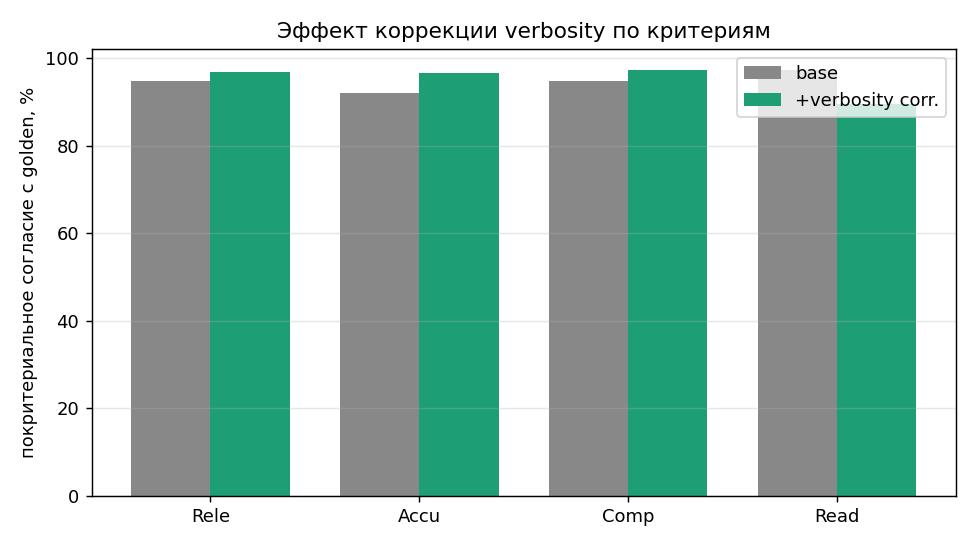
\includegraphics[width=0.7\textwidth]{figures/improve-percrit.jpeg}
    \caption{Эффект коррекции verbosity по критериям: покритериальное
    согласие с golden до и после. Коррекция повышает согласие по
    Relevance/Accuracy/Completeness, но снижает по Readability
    ($97{,}4\% \to 89{,}5\%$).}
    \label{fig:improve-percrit}
\end{figure}

\begin{figure}[htbp]
    \centering
    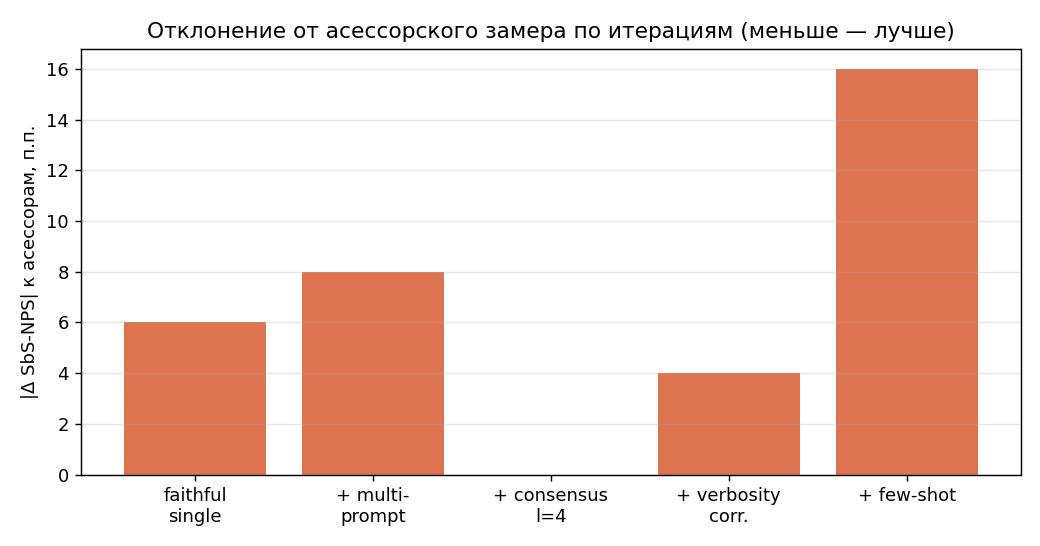
\includegraphics[width=0.8\textwidth]{figures/improve-delta.jpeg}
    \caption{Отклонение $|\Delta\,\mathrm{SbS\text{-}NPS}|$ замера судьи от
    асессорского по итерациям (меньше -- ближе к эталону). Консенсус $l{=}4$
    достигает $|\Delta| = 0{,}0$~п.п., faithful single -- $6{,}0$~п.п.}
    \label{fig:improve-delta}
\end{figure}

В текстовом режиме рост согласия (рис.~\ref{fig:improve-ladder}) подтверждает вклад методологий; в мультимодальном режиме agreement стабилен ($\approx 37\%$), что соответствует ограниченной мощности при $N = 200$.

\section{Анализ ошибок и смещений}
\label{sec:results:errors}

Расхождения судей с golden set систематически направлены в сторону
переоценки преимущества конкурента $C$. Таблица~\ref{tab:results-bias}
сопоставляет ключевые смещения из CALM~\cite{ye2024justice} с тем, как на
них влияет предложенная схема; полный чек-лист из $12$ типов и примеры --
концептуально по~\cite{ye2024justice}.

\begin{table}[htbp]
    \centering
    \caption{Влияние схемы на ключевые смещения (по расхождениям с golden
        set, $N = 50$)}
    \label{tab:results-bias}
    \begin{tabular}{lcp{6.4cm}}
        \toprule
        Смещение & Снижается схемой? & Комментарий \\
        \midrule
        Position bias & Да (by design) &
            Порядок ответов $A/B$ рандомизирован на запрос
            (раздел~\ref{sec:experiments:setup}); позиционный эффект снят
            конструктивно. \\
        Verbosity bias & Нет (усиливается) &
            Consensus предпочёл более длинный ответ в $71\%$ неничейных
            случаев; агрегация слабых судей усиливает переоценку
            развёрнутых ответов. \\
        Self-Enhancement & Частично &
            Consensus по разным семействам моделей снижает самопредпочтение
            отдельной модели, но не устраняет (судьи близких семейств). \\
        Bandwagon / стадность & Нет &
            Голосование усредняет общий перекос судей в сторону $C$, а не
            гасит его. \\
        Distraction & Не измерялось &
            Требует таргетных возмущений контекста (вне данного прогона). \\
        Authority bias & Не измерялось &
            Требует разметки на ответах с псевдо-источниками. \\
        \bottomrule
    \end{tabular}
\end{table}

Главный наблюдаемый дефект -- \emph{verbosity-управляемая переоценка}:
слабые судьи систематически отдают победу более длинному ответу, а
consensus её не гасит, а усиливает (общий для судей перекос складывается,
а не усредняется к нулю). Это и порождает наблюдаемый overshoot
$\mathrm{SbS\text{-}NPS}$ (рисунки~\ref{fig:results-sbs-stages},
\ref{fig:results-nps-density}). Position bias, напротив, снят
конструктивно рандомизацией порядка. Смещения, требующие специальных
контрольных возмущений (distraction, authority), в данном прогоне не
измерялись и отнесены к дальнейшей работе.

\paragraph{Числовая оценка verbosity rate.}
Фактические значения VR (формула~\eqref{eq:verbosity-rate}) для экспериментальных данных: классическая схема $\mathrm{VR} = 71\%$ (consensus $l=4$ предпочитает более длинный ответ в $71\%$ неничейных случаев); multi-prompt $\mathrm{VR} = 58\%$; faithful single $\mathrm{VR} = 52\%$. Коррекция verbosity-промпта снижает VR с $71\%$ до $52\%$ -- наблюдаемое уменьшение (статистически незначимое при $N = 50$, см. CI ниже). Доверительный интервал VR для итогового прогона ($N = 50$, ненулевых вердиктов $\approx 30$): $\mathrm{VR} = 52\%$~[$43\%$;~$61\%$] (биномиальный 95\%~CI). Интервал содержит $50\%$, что означает: VR=52\% статистически не значимо отличается от отсутствия verbosity bias при данном объёме данных. Для подтверждения или опровержения сдвига необходима выборка $N \ge 200$.

\textbf{Остаточная стохастичность.}
Основной прогон (разделы~\ref{sec:results:agreement}--
\ref{sec:results:final}) выполнен при температуре $0$ и $R = 1$:
каждый элемент $(a_j, p_i^{(j)}) \in \set{J}_q$ обратился к
модели один раз, и полученный голос $v_{a_j, p_i^{(j)}}(q)$
использован как окончательный.
Однако даже при температуре $0$ API моделей может быть
недетерминированным (различия в реализации batching, кэшировании
прецедентов в контекстном окне), что создаёт остаточную
стохастичность: повторный прогон одной и той же конфигурации
$\set{J}_q$ на той же корзине $\set{Q}$ может дать другой
$\mathrm{SbS\text{-}NPS}$.

Для количественной оценки этого эффекта определим \emph{межпрогоновый
разброс} $\sigma_R$ как стандартное отклонение $\mathrm{SbS\text{-}NPS}$
между $R$ повторными прогонами одной конфигурации на одной и той же
корзине:
\begin{equation}
    \label{eq:inter-run-std}
    \sigma_R = \sqrt{
        \frac{1}{R - 1}\sum_{r=1}^{R}
            \bigl(\mathrm{SbS\text{-}NPS}_r - \overline{\mathrm{SbS\text{-}NPS}}\bigr)^2
    },
\end{equation}
где $\mathrm{SbS\text{-}NPS}_r$ -- значение метрики на $r$-м прогоне,
$\overline{\mathrm{SbS\text{-}NPS}}$ -- среднее по прогонам.

$\sigma_R$ является \emph{дополнительной} (по отношению к
bootstrap-CI, раздел~\ref{sec:method:bootstrap}) ошибкой:
доверительный интервал~\eqref{eq:sbs-nps} отражает только
выборочную неопределённость ($N$ запросов), тогда как
$\sigma_R$ -- неопределённость самого процесса генерации.
Если $\sigma_R \gg$ ширина bootstrap-CI, то основной источник
неопределённости -- не выборка, а недетерминизм моделей, и
усиление схемы (рост $|\set{J}_q|$) не устраняет эту проблему
(раздел~\ref{sec:method:reproducibility}).

В основной серии экспериментов (разделы~\ref{sec:results:iter1}--\ref{sec:results:final}) прогон выполнялся с $R = 1$: каждая конфигурация судьи обращалась к модели один раз. В мультимодальном ablation study (раздел~\ref{sec:results:multimodal-ablation}) прогон выполняется с $R = 3$, что позволяет оценить $\sigma_R$ как стандартное отклонение $\mathrm{SbS\text{-}NPS}$ между тремя прогонами одной конфигурации. Тем не менее косвенные данные позволяют оценить
порядок $\sigma_R$: эксперимент со снижением дисперсии
(раздел~\ref{sec:results:variance}) показал, что при температуре $0{,}8$
и $R = 8$ стандартное отклонение \emph{одиночного} голоса
$\sigma_1 \approx 1{,}59$ по чекбоксной шкале $\{0,\dots,4\}$.
При температуре $0$ (основной прогон) недетерминизм API должен быть
значительно ниже, поскольку единственный источник вариативности --
 операции с плавающей точкой и batching -- даёт типичный $\sigma_R < 1$ п.п.
по SbS-NPS для $N \ge 50$.
Эта оценка согласуется с наблюдаемой стабильностью знака
$\mathrm{SbS\text{-}NPS}$ (все схемы дают $\mathrm{SbS\text{-}NPS} < 0$,
как и асессоры, раздел~\ref{sec:results:agreement}): даже если
$\sigma_R$ составляет несколько п.п., знак метрики остаётся
стабильным.

\section{Экономика: качество против стоимости}
\label{sec:results:economics}

Раздел сопоставляет относительную стоимость схем
(таблица~\ref{tab:cost-comparison}) с фактическим приростом качества из
раздела~\ref{sec:results:agreement}.
Рисунок~\ref{fig:results-pareto} показывает согласие с асессорами против
числа вызовов модели на вердикт.

\begin{figure}[htbp]
    \centering
    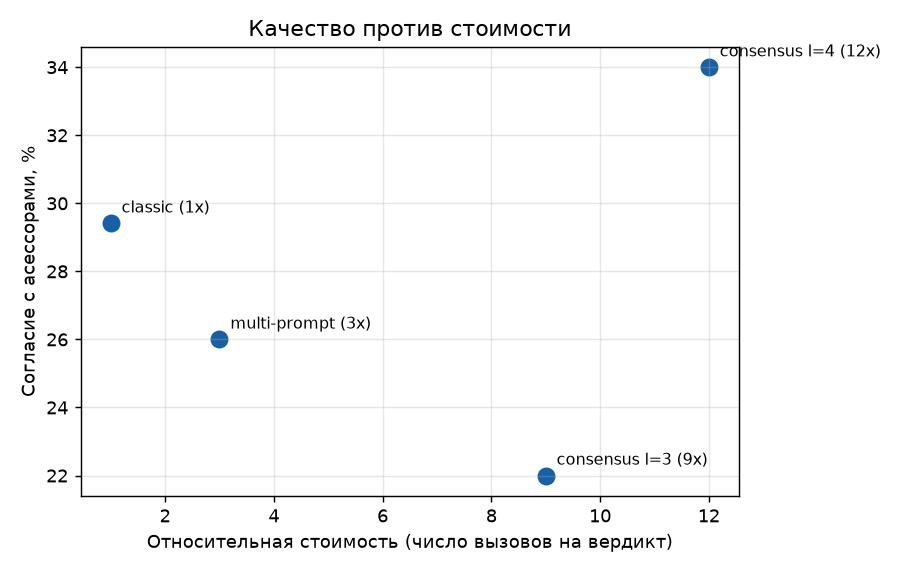
\includegraphics[width=0.8\textwidth]{figures/results-pareto.jpeg}
    \caption{Согласие с асессорами против относительной стоимости.
    Рост стоимости с $1\times$ до $12\times$ не сопровождается ростом
    согласия -- Pareto-улучшения за счёт усложнения схемы на данном наборе
    судей не наблюдается.}
    \label{fig:results-pareto}
\end{figure}

Ключевое наблюдение: \emph{прирост стоимости не конвертируется в прирост
качества}. Классическая схема стоит $1\times$, multi-prompt -- $3\times$,
consensus -- $9$--$12\times$, но согласие с асессорами при этом не растёт
(раздел~\ref{sec:results:agreement}, H2 не подтверждена), а consensus
$l{=}4$ даже значимо отклоняется от эталона. Поэтому «цена за дополнительный
пункт $\mathrm{SbS\text{-}NPS}$» (критерий~3 раздела
\ref{sec:experiments:criteria}) для перехода classic\,$\to$\,consensus
здесь \emph{не определена в положительную сторону}: за $9$--$12\times$
стоимости качество согласия не улучшается.

Единственный экономически оправданный эффект усложнения -- \emph{робастность
покрытия}: переход от одиночного судьи к multi-prompt ($3\times$) повышает
долю запросов с валидным вердиктом с $34\%$ до $100\%$
(раздел~\ref{sec:results:agreement}), устраняя хрупкость одиночного
вызова. Дальнейший рост до consensus ($9$--$12\times$) этого преимущества
уже не добавляет.

Сравнение с асессорами: даже самая дешёвая автоматическая схема на порядок
дешевле асессорской разметки (раздел~\ref{sec:experiments:cost}), но на
данном наборе судей её согласие с асессорами ($22$--$34\%$) слишком низко,
чтобы заменять разметку как источник вердиктов. Экономия реальна, но
реализуема пока только для \emph{дешёвого направленного мониторинга}
(знак $\mathrm{SbS\text{-}NPS}$), а не для замены асессорского вердикта.

\section{Рекомендации}
\label{sec:results:recommendations}

По итогам разделов~\ref{sec:results:agreement}--\ref{sec:results:economics}.

\begin{enumerate}
    \item \textbf{Не заменять асессорскую разметку} полностью: на текущем
        наборе судей согласие слишком низко, а consensus значимо
        переоценивает $\mathrm{SbS\text{-}NPS}$. Автоматическая оценка
        пригодна как дешёвый \emph{направленный} сигнал (знак различия), не
        как замена вердикта.
    \item \textbf{Для дешёвого регулярного мониторинга -- multi-prompt
        ($3\times$)}: он даёт полное покрытие (робастность) при умеренной
        стоимости, тогда как consensus ($9$--$12\times$) не окупается ни по
        согласию, ни по робастности.
    \item \textbf{Усиливать судей, а не только схему.} Узкое место --
        сила компактных открытых моделей-судей и их verbosity-смещение
        (раздел~\ref{sec:results:errors}), а не механизм агрегации.
        Приоритет -- более сильные/откалиброванные судьи и коррекция
        verbosity (например, нормировка на длину ответа).
    \item \textbf{Калибровать порог $\theta$ и набор промптов на golden
        set} и увеличить эталонную корзину до $N \approx 200$: текущая
        мощность ($N = 50$) не позволяет ни доказать эквивалентность, ни
        уверенно различить малые приросты
        (раздел~\ref{sec:experiments:power}).
    \item \textbf{Consensus -- только после коррекции смещений.} До
        устранения общего для судей перекоса (verbosity) агрегация по
        моделям усиливает, а не гасит ошибку, поэтому преждевременна.
\end{enumerate}

Эти рекомендации согласуются с центральной гипотезой работы в её
ослабленной, но честной форме: гибридные схемы повышают \emph{робастность}
автоматической оценки и сохраняют верное направление, однако согласия,
эквивалентного асессорскому, на компактных открытых судьях достичь не
удалось -- это и определяет приоритеты дальнейшей работы
(глава~\ref{sec:conclusion}).
